
\section*{Problem 2: Report on Player 15411's Outfield Defense}
\label{sec:expts}

The following evaluation is based on 375 hits for which player 15411 (henceforth, "the player") was identified as the primary fielder. The player's only recorded position for these 375 hits is center field.

The player began the 2023 season at level B and was transferred to level A about a month later (on May 5, 2023). The player was responsible for 237 air outs over the course of the season.

\subsection{Bottom Line Up Front}

The player is a strong outfield defender capable of taking away big hits from the opposition. The player made the adjustment to level A smoothly and maintained a high level of play throughout the season.

\subsection{Overall Performance}
\label{sec:overallperformance}

The player's outfield performance during the 2023 season was in the 83rd percentile among qualified outfielders (at least 10 air outs during the season) in terms of mean air outs above expected (mAOAE). This statistic represents how much more likely a player is to catch a given ball than the average player. The player had a mAOAE of 0.026, so they were about 2.6 percentage points more likely to catch a given ball than the average player.

That said, this number conceals significant variation in the player's performance based on the type of ball which was hit into center field. As shown in Figure \ref{fig:hittype}, the player was significantly above average at catching hits classified as a barrel or solid contact, and below average at catching hits classified as a flair or burner.

\begin{figure}[htb]
    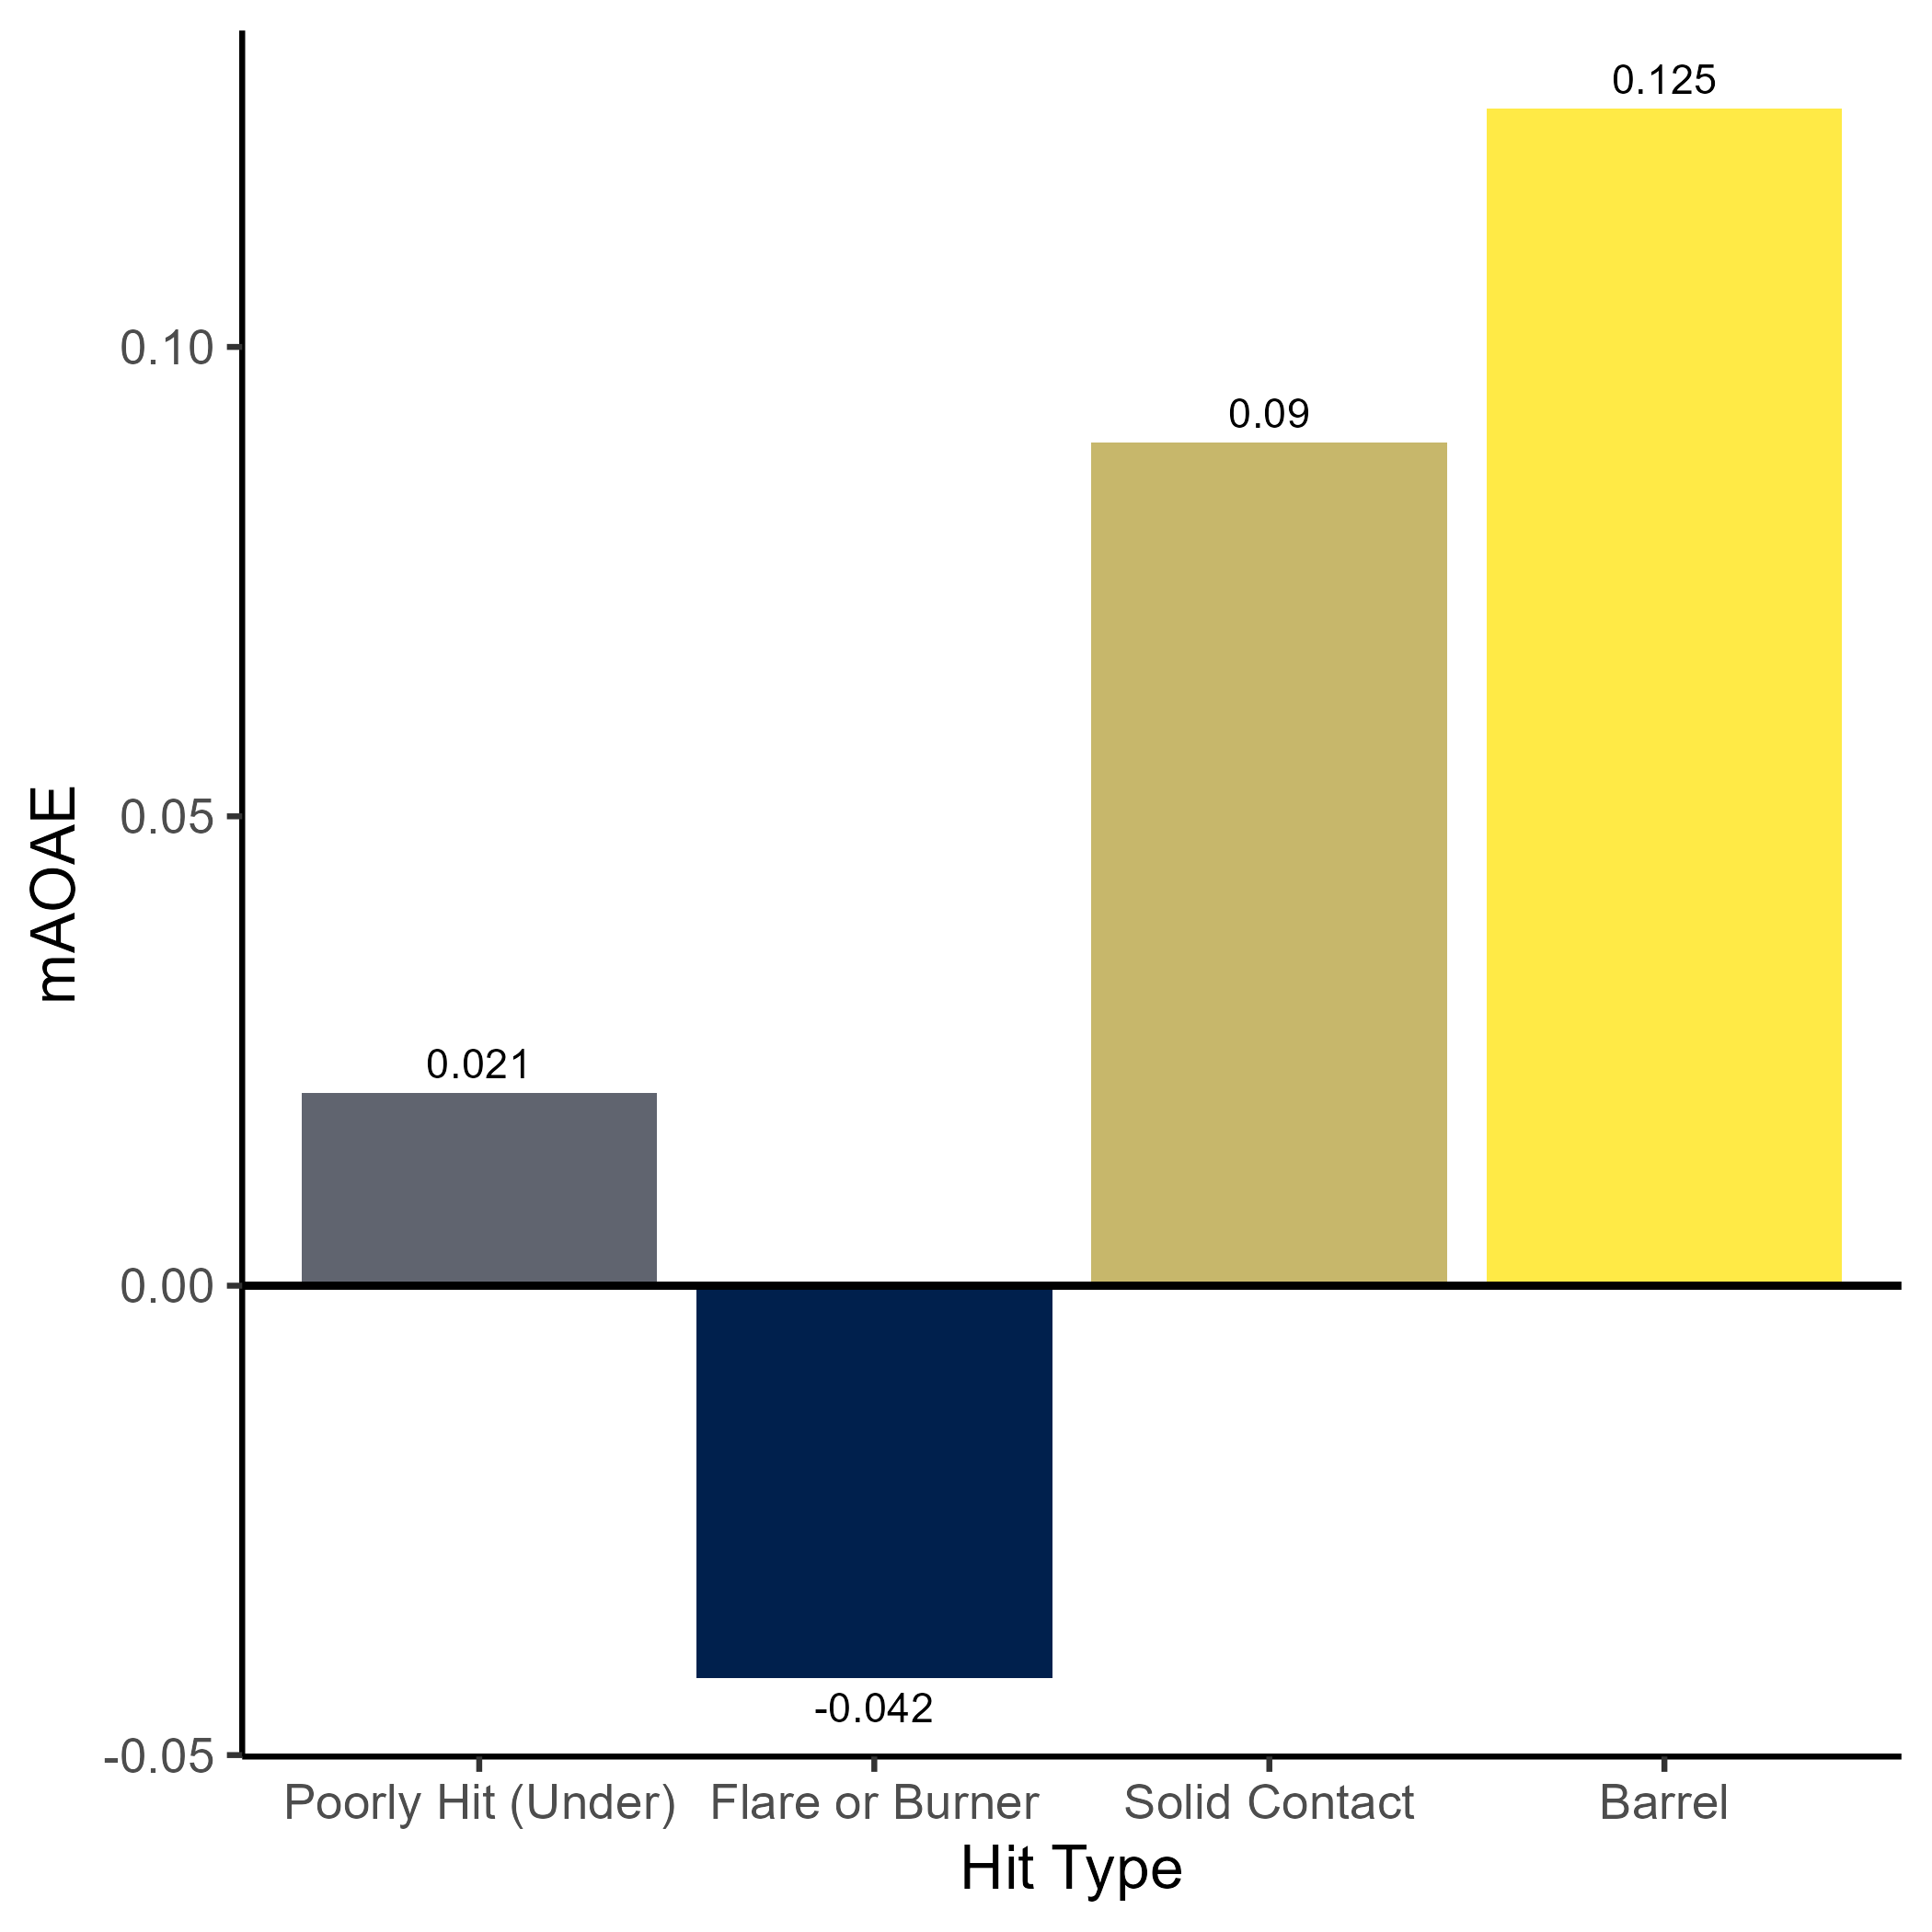
\includegraphics[width = 0.47\textwidth]{../../output/figs/hit_type_15411.png}
    \caption{Player 15411's Fielding Performance Against Hit Type}
    \label{fig:hittype}
\end{figure}

This has significant implications for fielding performance. More than half of barrels result in a home run, and nearly 80 percent result in a base hit \cite{metzelaar}. Solid hits fall just short of being classified as a barrel, but they are excellent at generating extra-base hits. In short, this player is capable of taking away the most valuable hits at a high rate.

\subsection{Adjustment to Level A}
\label{sec:adjustment}

The player's best defensive month of the season was the first month, which the player spent most of at level B. However, a battery of statistical tests do not show any evidence that the player's performance significantly declined after being transferred to level A. This can be seen in Figure \ref{fig:scores}, where the vertical line represents the day on which the player was transferred to level A.

\begin{figure}[htb]
    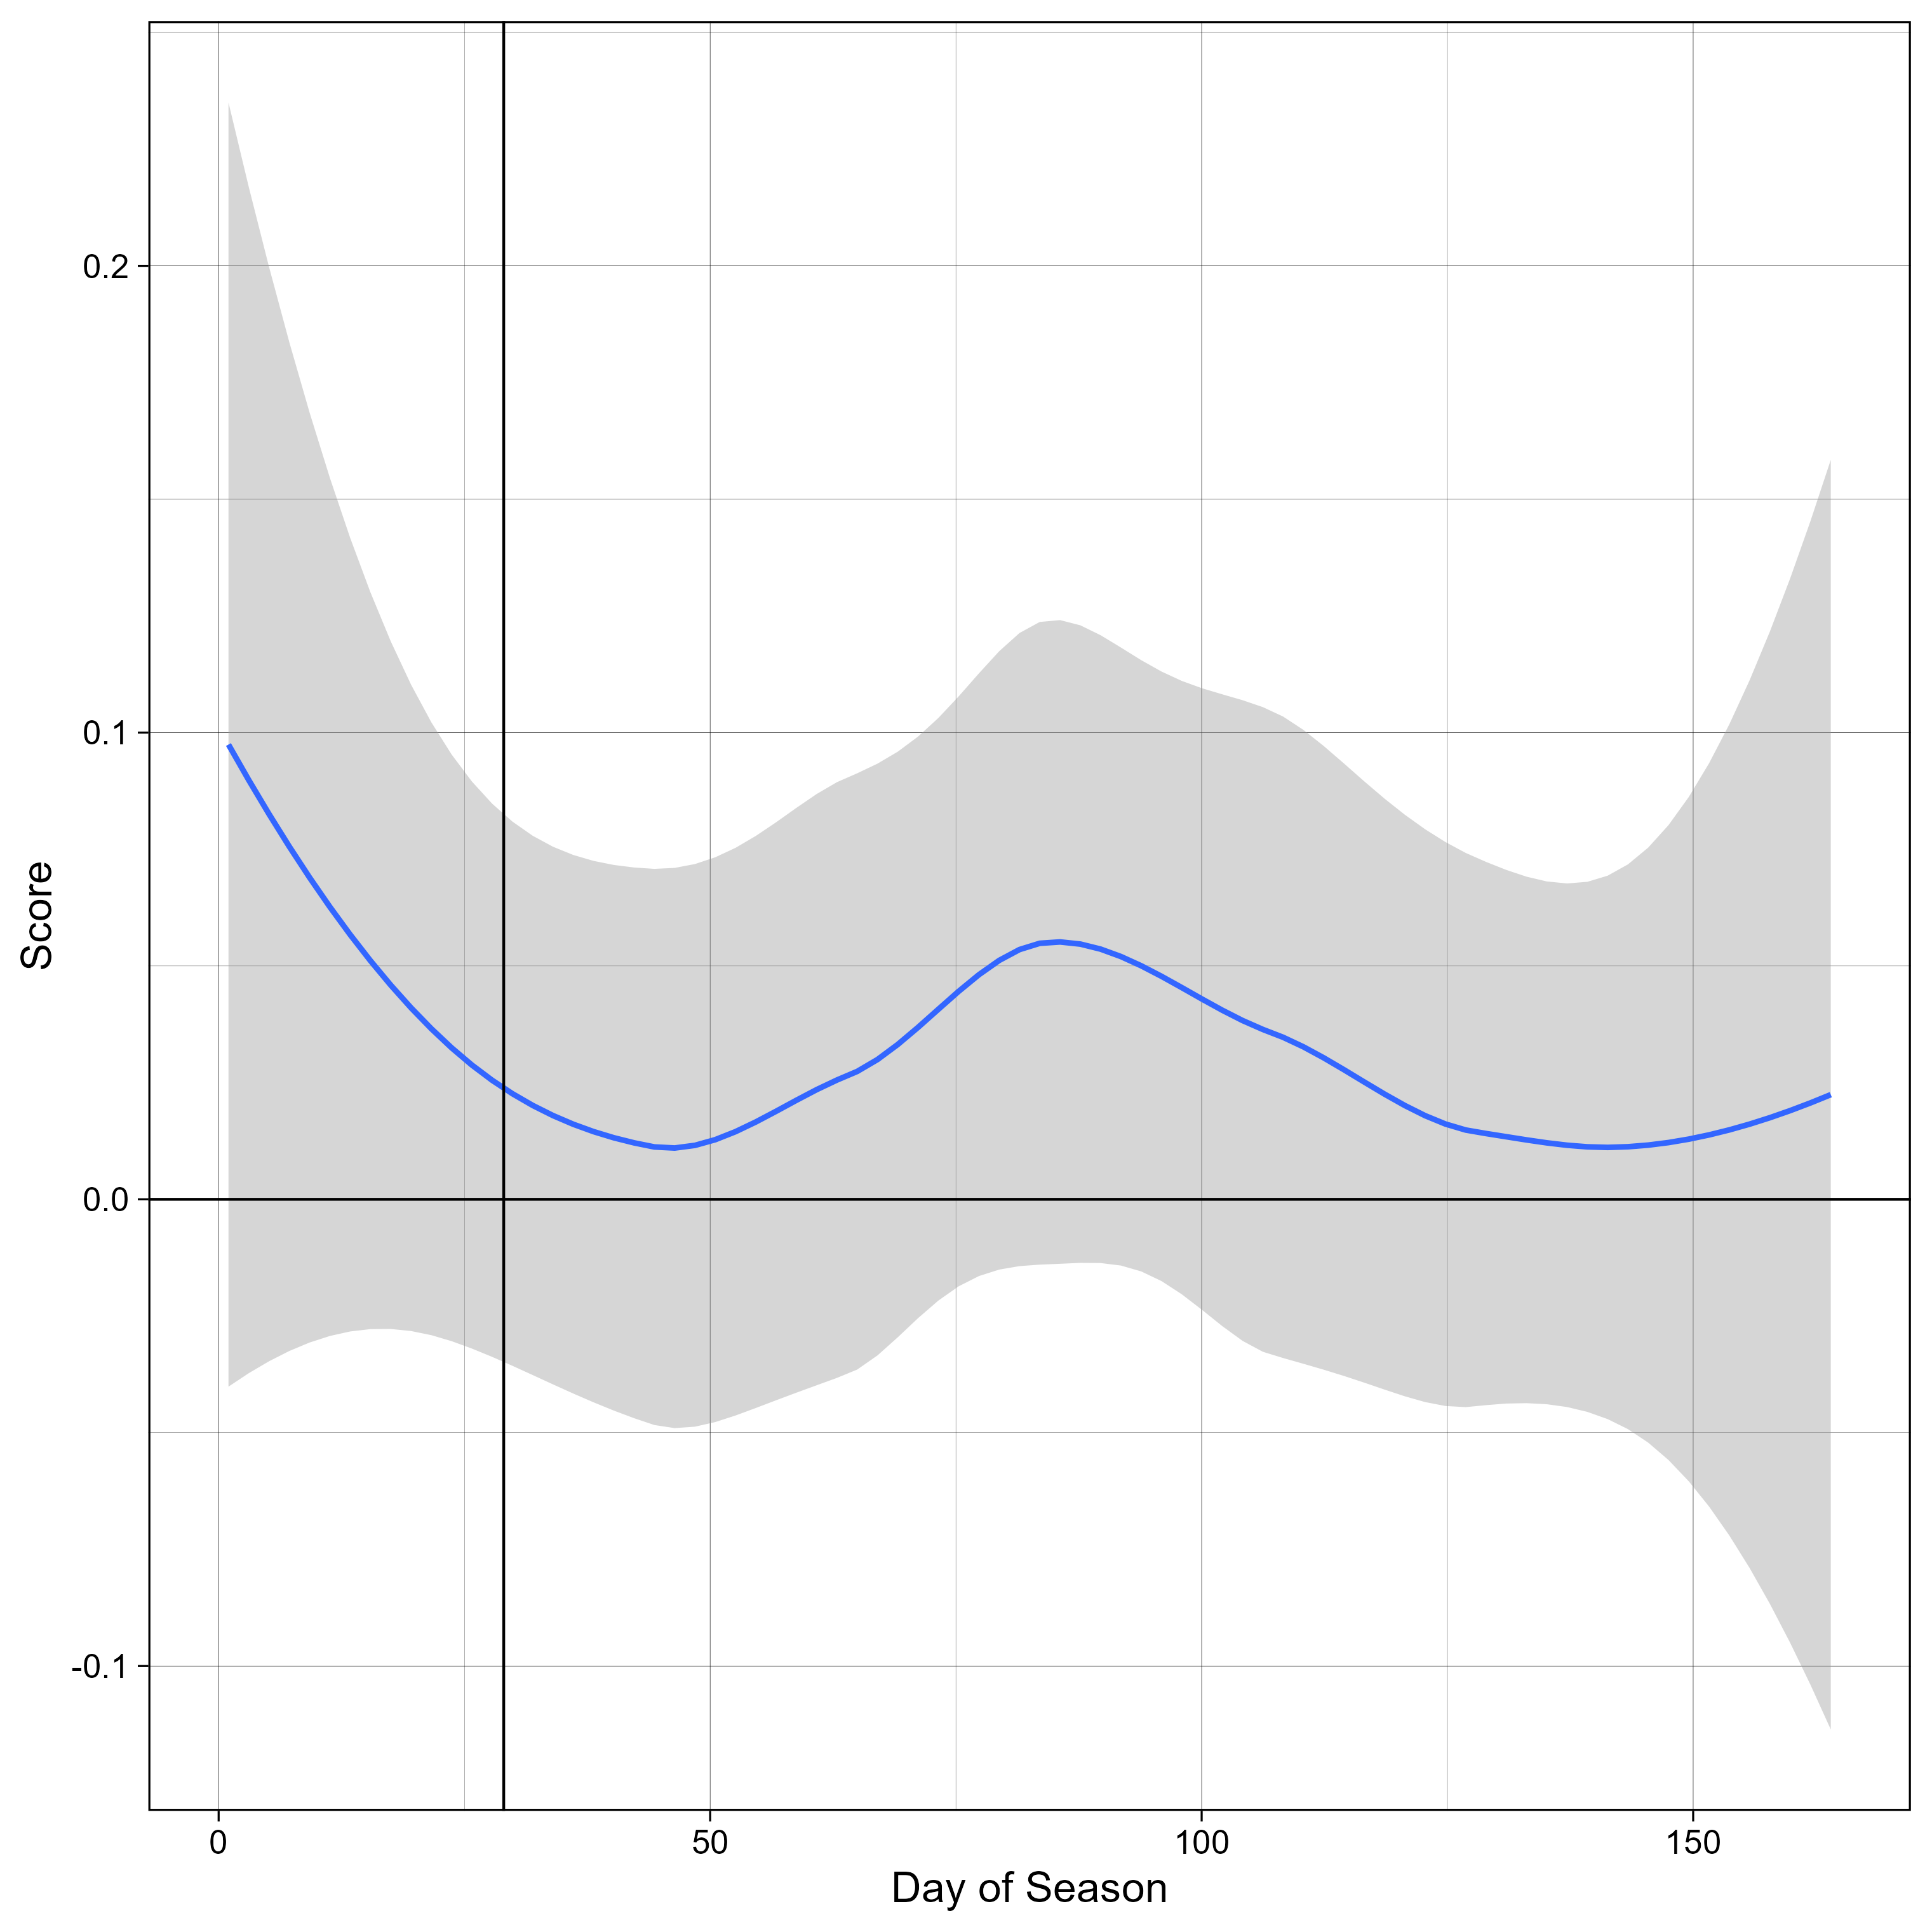
\includegraphics[width = 0.47\textwidth]{../../output/figs/score_plot_15411.png}
    \caption{Player 15411's Fielding Score over Time}
    \label{fig:scores}
\end{figure}